\section{Esercizio 4}

Si calcoli con un metodo MC l'integrale $ \displaystyle\int_{-1}^{+1}(x^5+x^4)\mathop{dx}$ e si discutano le possibili tecniche di riduzione della varianza.

\bigskip\[* * * \] \smallskip

\noindent Consideriamo il generico integrale $ \displaystyle
\mathcal{S} = \int_a^b f(x) \mathop{dx}$, con $b>a \in \mathbb{R}$ e $f(x)$ funzione integrabile di variabile reale.\\

\noindent Definendo $g(x)$ come la densità di probabilità uniforme nell'intervallo $[a,b]$ possiamo riscrivere l'integrale $\mathcal{S}$ come

\begin{equation*}
(b-a)\int_{\mathbb{R}} f(x) g(x) \mathop{dx} = (b-a)\int_{\mathbb{R}}\mathbb{I}_{[a,b]}\frac{f(x)}{b-a}\mathop{dx} = \int_a^b f(x) \mathop{dx} = \mathcal{S},
\end{equation*}

\noindent e quindi definire un valore medio $F$ tale per cui $\mathcal{S} = (b-a)F$:

\begin{equation*}
F = \int_{\mathbb{R}}f(x)g(x)\mathop{dx}.
\end{equation*}

\noindent Per la \textit{legge dei grandi numeri} (Cfr.~\figurename~\ref{fig:MCHist}) possiamo inoltre costruire uno stimatore per $F$ utilizzando un generatore di numeri pseudo-casuali distribuiti secondo $g(x)$. Indicata con $\{x_i\}$ la sequenza generata e con $N$ la sua numerosità scriviamo allora:

\begin{equation}
\hat{F}_N = \frac{1}{N} \sum_{i=1}^{N}f(x_i),\quad \lim_{N\to\infty} (b-a)\hat{F}_N= \mathcal{S}.
\label{eq:MCstandard}
\end{equation}

\noindent Per $N$ finito possiamo anche valutare l'incertezza sulla stima di $\mathcal{S}$ per mezzo di uno stimatore della varianza di $\hat{F}_N$:

\begin{align}
\hat{S}_N &= \sqrt{\frac{1}{N-1} \left(\sum_{i=1}^{N}\bigl[(f(x_i))^2\bigr] - \bigl[\hat{F}_N\bigr]^2\right)}\\
\nonumber\\
\mathcal{S} &= (b-a)\left(\hat{F}_N \pm \frac{\hat{S}_N}{\sqrt{N}}\right)
\end{align}

\begin{figure}
	\centering
	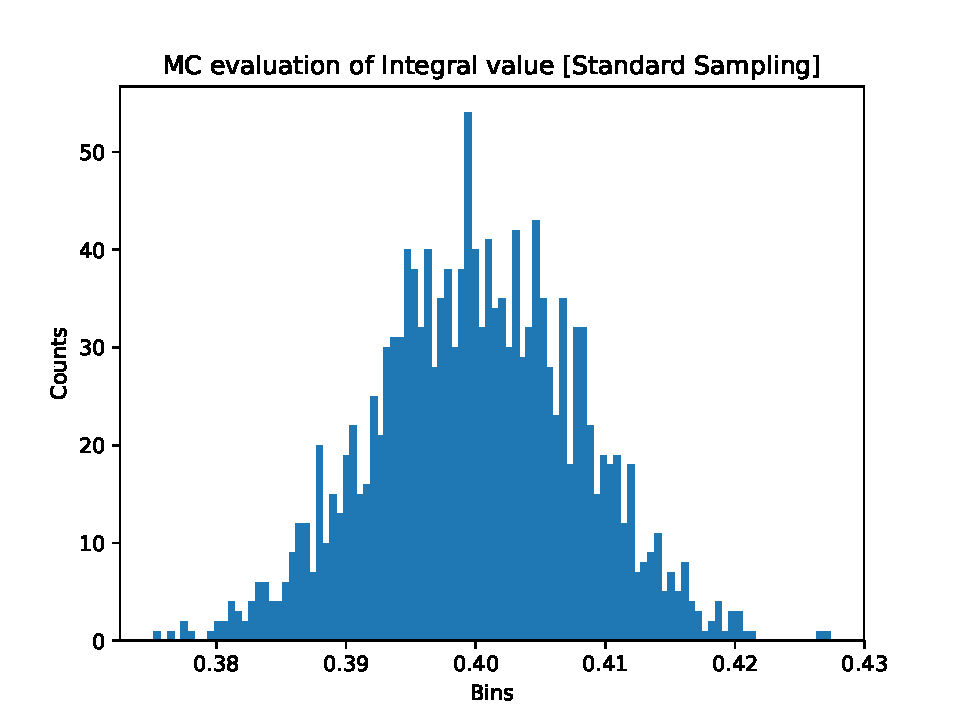
\includegraphics[width=.7\textwidth]{Immagini/Es4Hist.pdf}
	\caption{Istogramma relativo alla distribuzione generata per la variabile casuale $\mathcal{S}$ nell'implementazione standard del metodo Montecarlo, con $N=10^4$ eventi generati. \`E evidente che si tratta in buona approssimazione di una distribuzione normale, in accordo con la legge dei grandi numeri.}
	\label{fig:MCHist}
\end{figure}

\noindent Risulta subito evidente che la dipendenza da $N$ dell'incertezza non è particolarmente felice: pur garantendo uno stimatore non biassato nel limite $N\to\infty$, la convergenza è molto lenta producendo quindi algoritmi sostanzialmente inefficienti. Da tale considerazione nasce dunque l'interesse per algoritmi che riducano la varianza rispetto al metodo definito dalla (\ref{eq:MCstandard}), senza ovviamente produrre bias sul valor medio. Di seguito illustriamo due diverse tecniche di riduzione della varianza: \emph{Importance Sampling} e \emph{Stratified Sampling}.

\begin{description}
	
	\item[\quad\quad\! Importance Sampling]\quad\\
	Sia una generica densità di probabilità $p(x)\!: [a,b]\mapsto\mathbb{R}^+,\int_{a}^{b}p(x)\mathop{dx} = 1$. Se in $[a,b]$ tale densità si annulla al più in un sottoinsieme di punti di misura nulla possiamo riscrivere l'integrale $\mathcal{S}$ come:
	
	\begin{equation*}
	\mathcal{S} = \int_{a}^{b} \frac{f(x)}{p(x)}p(x)\mathop{dx} \simeq \frac{1}{N}\sum_{i=1}^{N}\frac{f(x_i)}{p(x_i)},\enspace \text{dove le } \{x_i\} \text{ sono distribuite secondo } p(x).
	\end{equation*}
	
	In questa situazione possiamo scrivere la varianza teorica di $\mathcal{S}$ come
	
	\begin{equation}
	\sigma^2[\,\mathcal{S}\,] = \frac{\sigma^2[\,f/p\,]}{N},
	\label{eq:ImportanceSampling}
	\end{equation}
	
	e osservare che laddove la densità $p(x)$ risulti proporzionale a $f(x)$ (in $[a,b]$!) la varianza $\sigma^2[\,f/p\,] = \sigma^2[\,\text{const.}]$ risulterà identicamente nulla. Senza pretese di rigore possiamo allora intuire che, fissato $N$, quanto più "$p(x)$ sarà simile a $f(x)$", tanto più la varianza di $\mathcal{S}$ tenderà a ridursi.\\
	Naturalmente nel caso generale risulta piuttosto difficile generare numeri casuali secondo una distribuzione simile alla funzione desiderata, per cui sostanzialmente si cerca di scrivere l'integrando come una combinazione lineare di densità note e si calcolano separatamente i rispettivi contributi a $\mathcal{S}$ e alla sua varianza. Nel nostro caso si è partizionato l'intervallo $[a,b]$ in maniera tale da poter approssimare la $f(x)$ con la somma di una distribuzione \emph{triangolare} e di una distribuzione \emph{beta}, con supporti disgiunti (Cfr.~\figurename~\ref{fig:MCImpSampl} e Listato~\ref{list:ImpSampling}).
		
	\item[\quad\quad\! Stratified Sampling]\quad\\
	Si tratta di un metodo basato sulla sola proprietà additiva degli integrali: considerato un punto $c\in[a,b]$ si ha analiticamente
	
	\begin{equation*}
	\int_{a}^{b} f(x)\mathop{dx} = \int_{a}^{c} f(x)\mathop{dx} + \int_{c}^{b} f(x)\mathop{dx}.
	\end{equation*}
	
	Tuttavia può essere dimostrato che partizionando l'intervallo $[a,b]$ in sottointervalli sui quali applicare un calcolo Montecarlo "standard" (i.e.~con estrazione di numeri casuali distribuiti uniformemente) si ottiene in generale una varianza totale differente rispetto al medesimo calcolo valutato sull'intervallo complessivo, a parità di estrazioni totali. In particolare si può allora ottimizzare la scelta di come ripartire nei sottointervalli il numero di eventi generati, al fine di minimizzare la varianza complessiva del calcolo: in ragione della (\ref{eq:ImportanceSampling}) possiamo argomentare che sarà preferibile campionare maggiormente le regioni in cui la funzione integranda varia più rapidamente, ossia laddove si discosti maggiormente da una densità uniforme. Nel nostro caso (Listato~\ref{list:StratSampling}) abbiamo definito sette sottointervalli con campionamento crescente da sinistra a destra, per un totale di $N$ eventi generati: in tal modo il calcolo risulta confrontabile con l'implementazione standard (Listato~\ref{list:MC}).
	
\end{description}

\noindent In linea di massima ci aspettiamo che l'\textit{Importance Sampling} risulti più efficiente nel ridurre la varianza rispetto allo\textit{ Stratified Sampling}, a patto che sia possibile approssimare la funzione integranda in combinazioni lineari di densità di probabilità elementari (i.e. semplici da generare). Nel caso generale invece un campionamento stratificato resta senz'altro l'opzione più flessibile e immediata da implementare.\\

\[* * * \] \smallskip

\noindent Di seguito riportiamo i risultati ottenuti con il calcolo \textit{Standard} (Listato~\ref{list:MC}), con\textit{ Importance Sampling} (Listato~\ref{list:ImpSampling}) e con \textit{Stratified Sampling} (Listato~\ref{list:StratSampling}), in termini di media e deviazione standard delle gaussiane generate per la variabile aleatoria $\mathcal{S}$. In tutti i casi sono stati estratti complessivamente $10^4$ campioni.
 
 \bgroup
 \def\arraystretch{2}
 \begin{center}
 	\begin{tabular}{r||c|c}
 	$ \mathcal{S} = \int_{-1}^{+1}(x^5+x^4)\mathop{dx}$ & \textit{Media Campionaria} & \textit{Deviazione Standard Campionaria }\\  \hline
 		\textit{Standard Sampling }& 0.4032560803645552  & 8.077310205890864 $\times \,\,10^{-3}$\\ 
 		\textit{Importance Sampling} & 0.3989493411116131 & 1.113214189831381 $\times\,\, 10^{-3}$\\ 
 		\textit{Stratified Sampling} & 0.4019606513273493 & 1.462526565299890 $\times \,\,10^{-3}$\\
 	\end{tabular}
 \end{center}
 \egroup
 
 \noindent Risulta innanzitutto evidente che i valori medi delle tre stime approssimano bene il valore analitico $\mathcal{S}=0.4$. Inoltre risultano tra loro compatibili ({entro meno di}~$2\sigma$), a riprova del fatto che le tecniche di riduzione della varianza utilizzate non traslano il valor medio dell'integrale. Osserviamo infine come la varianza campionaria diminuisce di un ordine di grandezza passando da \textit{Standard Sampling} a \textit{Stratified Sampling} e di quasi due ordini di grandezza utilizzando l'\textit{Importance Sampling}. Tali risultati soddisfano appieno le nostre aspettative.

\begin{figure}
	\centering
	\caption{Costruzione dell'\emph{Importance Sampling} per il calcolo di $\mathcal{S}$. Le due distribuzioni elementari utilizzate sono state moltiplicate per opportune costanti in modo da evidenziare quanto efficacemente riproducono la funzione~data.}
	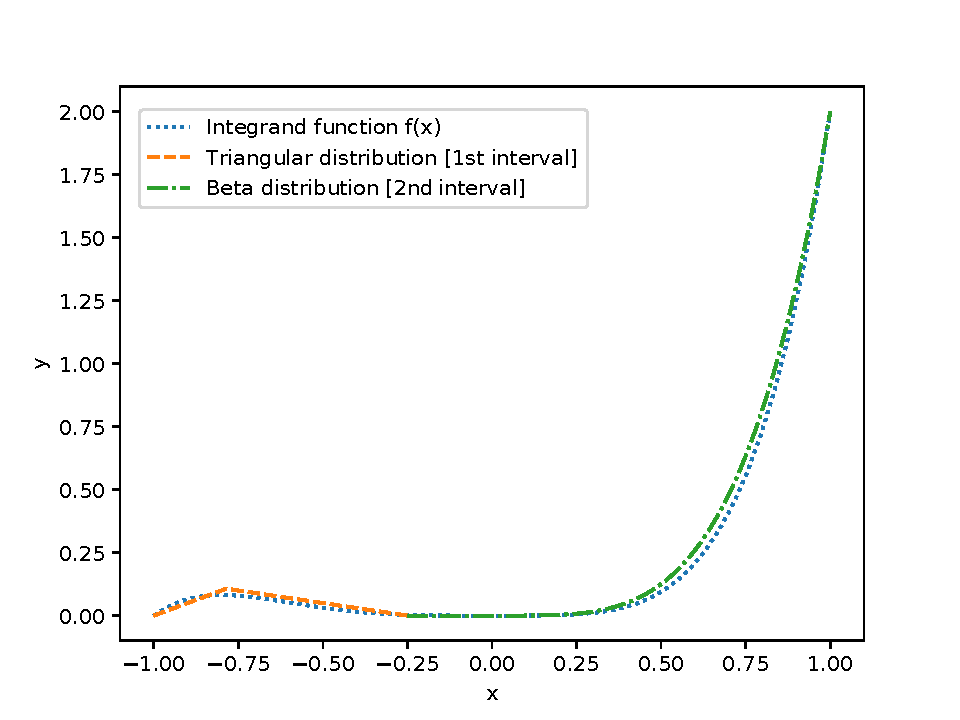
\includegraphics[width=.77\textwidth, trim={0 .3cm 0 1.3cm},clip]{Immagini/Es4ImportanceSampling.pdf}
	\label{fig:MCImpSampl}
\end{figure}

\newpage

\begin{lstlisting}[language=python, style=Pystyle, caption=\texttt{Python} code for Standard Montecarlo Calculation, label=list:MC, 	captionpos=t]
import numpy as np
import matplotlib.pyplot as plt
import math

## Integrand function
def f(x): return x**5+x**4

## Integration interval
a =-1.0
b = 1.0

## Number of random number generations
n = 10000

## Standard MC implementation
h=[]
for k in range(1,1500):  

	x=np.random.uniform(a,b,n)  # [a,b]=[-1.0,1.0]
	eval_funct=f(x) 
	h.append((b-a)*np.sum(eval_funct)/(n))

S=(b-a)*(np.sum(eval_funct))/n
n=10000.0
mu_camp=(np.sum(eval_funct))/n
var_camp=1/(n-1)*np.sum((eval_funct-mu_camp)**2)
var=(b-a)**2*(1/n)*var_camp

print (S,'Integral Mean with Standard MC')
print (var,'Variance with Standard MC')
print(sqrt(var), 'Standard Deviation with Standard MC')

## Plotting a histogram of the generated gaussian
hist,bin_edges=np.histogram(h,bins=100)
plt.figure()
plt.hist(h,bin_edges)
plt.xlabel('Bins')
plt.ylabel('Counts')
plt.title('MC evaluation of Integral value [Standard Sampling]')
axes=plt.gca()

plt.show()
\end{lstlisting}

\begin{lstlisting}[language=python, style=Pystyle, caption=\texttt{Python} code for Importance Sampling Montecarlo Calculation, label=list:ImpSampling, 	captionpos=t]
import numpy as np
import matplotlib.pyplot as plt
import math
from scipy.stats import triang
from scipy.stats import beta

## Integrand function
def f(x): return x**5+x**4

x=np.linspace(-1,1,endpoint=True,dtype=float)
plt.plot(x,f(x),'.')

## 1st Interval: Triangular-approximation
s=np.linspace(-1,-0.25,50)
plt.plot(s,0.04*triang.pdf(s,0.2/0.7,a,b-a), '--')
a=-1
b=-0.25
n1=50
x1=np.random.triangular(a,-0.8,b,n1)  
eval_funct1=f(x1) 
y1=triang.pdf(x1,0.2/0.7,a,b-a)
n1=n1*1.0

i1=(1/n1)*np.sum(eval_funct1/y1)

mu_camp1=(np.sum(eval_funct1/y1))/n1
var_camp1=1/(n1-1)*np.sum((eval_funct1/y1-mu_camp1)**2)
var1=(1/n1)*var_camp1

## 2nd Interval: Beta-approximation
k=np.linspace(-0.25,1,100)
plt.plot(k,0.4*beta.pdf(k,5,1), '-.')

n2=9950
x2=beta.rvs(5,1,size=n2)  
eval_funct2=f(x2) 
y2=beta.pdf(x2,5,1)                     

n2=n2*1.0
i2=(1/n2)*np.sum(eval_funct2/y2)

mu_camp2=(np.sum(eval_funct2/y2))/n2
var_camp2=1/(n2-1)*np.sum((eval_funct2/y2-mu_camp2)**2)
var2=(1/n2)*var_camp2

## Results
print(i1+i2,'Integral Mean with Importance Sampling')
print(var1+var2,'Total Variance with Importance Sampling')
print(sqrt(var1+var2), 'Total Standard Deviation with Importance Sampling')
plt.xlabel('x')
plt.ylabel('y')
plt.show()
\end{lstlisting}

\begin{lstlisting}[language=python, style=Pystyle, caption=\texttt{Python} code for Stratified Sampling Montecarlo Calculation, label=list:StratSampling, 	captionpos=t]
import numpy as np
import math

## Integrand function
def f(x): return x**5+x**4

## 1st Interval 
a=-1.0
b=-0.4
n1=100
x1=np.random.uniform(a,b,n1)  # [a,b]=[-1.0,-0.4]
k=np.linspace(0.35,1,50)
eval_funct1=f(x1)
n1=n1*1.0 
i1=(b-a)*(np.sum(eval_funct1)/n1) # mean
mu_camp1=(np.sum(eval_funct1))/n1
var_camp1=(1/(n1-1))*np.sum((eval_funct1-mu_camp1)**2)  # variance
var1=(b-a)**2*(1/n1)*var_camp1

## 2nd Interval 
a=-0.4
b=0.4
n2=100
x2=np.random.uniform(a,b,n2)  # [a,b]=[-0.4,0.4]
eval_funct2=f(x2) 
n2=n2*1.0
i2=(b-a)*(np.sum(eval_funct2)/n2) # mean
mu_camp2=(np.sum(eval_funct2))/n2
var_camp2=1/(n2-1)*np.sum((eval_funct2-mu_camp2)**2)  # variance
var2=(b-a)**2*(1/n2)*var_camp2

## 3rd Interval 
a=0.4
b=0.6
n3=800
x3=np.random.uniform(a,b,n3)  # [a,b]=[0.4,0.6]
eval_funct3=f(x3) 
n3=n3*1.0
i3=(b-a)*(np.sum(eval_funct3)/n3) # mean
mu_camp3=(np.sum(eval_funct3))/n3
var_camp3=1/(n3-1)*np.sum((eval_funct3-mu_camp3)**2)  # variance
var3=(b-a)**2*(1/n3)*var_camp3

## 4th Interval 
a=0.6
b=0.7
n4=1000
x4=np.random.uniform(a,b,n4)  # [a,b]=[0.6,0.7]
eval_funct4=f(x4) 
n4=n4*1.0
i4=(b-a)*(np.sum(eval_funct4)/n4) # mean
mu_camp4=(np.sum(eval_funct4))/n4
var_camp4=1/(n4-1)*np.sum((eval_funct4-mu_camp4)**2)  # variance
var4=(b-a)**2*(1/n4)*var_camp4

## 5th Interval 
a=0.7
b=0.8
n5=1500
x5=np.random.uniform(a,b,n5)  # [a,b]=[0.7,0.8]
eval_funct5=f(x5) 
n5=n5*1.0
i5=(b-a)*(np.sum(eval_funct5)/n5) # mean
mu_camp5=(np.sum(eval_funct5))/n5
var_camp5=1/(n5-1)*np.sum((eval_funct5-mu_camp5)**2)  # variance
var5=(b-a)**2*(1/n5)*var_camp5

## 6th Interval 
a=0.8
b=0.9
n6=3000
x6=np.random.uniform(a,b,n6)  # [a,b]=[0.8,0.9]
eval_funct6=f(x6) 
n6=n6*1.0
i6=(b-a)*(np.sum(eval_funct6)/n6) # mean
mu_camp6=(np.sum(eval_funct6))/n6
var_camp6=1/(n6-1)*np.sum((eval_funct6-mu_camp6)**2)  # variance
var6=(b-a)**2*(1/n6)*var_camp6

## 7th Interval 
a=0.9
b=1.0
n7=3500
x7=np.random.uniform(a,b,n7)  # [a,b]=[0.9,1]
eval_funct7=f(x7) 
n7=n7*1.0
i7=(b-a)*(np.sum(eval_funct7)/n7) # mean
mu_camp7=(np.sum(eval_funct7))/n7
var_camp7=1/(n7-1)*np.sum((eval_funct7-mu_camp7)**2)  # variance
var7=(b-a)**2*(1/n7)*var_camp7

## Results
print(n1+n2+n3+n4+n5+n6+n7,'Check on total number of generations [has to be 10^4]')
S=i1+i2+i3+i4+i5+i6+i7
print(S,'Total mean for S, with Stratified Sampling')
var=var1+var2+var3+var4+var5+var6+var7
print(var ,'Total variance for S, with Stratified Sampling')
dev = sqrt(var)
print(dev ,'Total standard deviation for S, with Stratified Sampling')
\end{lstlisting}

\newpage